\documentclass[../../thesis.tex]{subfiles}

\begin{document}
Our work, as well as out models can be divided into two stages. Firstly we investigate the effect of non-contrastive SSL on a proven tokenization model, VQVAE \cite{VQVAE}, with the goal of learning more expressive representations. The expressiveness is measured in terms of the models ability to reconstruct unseen data, as well at the performance of learned latent representations on a downstream classification task. The SSL models we consider are, as introduced in section 3 \todo{make hyperlink}, BarlowTwins and VIbCReg.\\\\

Secondly we investigate the effects of NC-VQ-VAE on prior learning by training a MaskGIT model on top of the tokenization models.\\\\

Additionally we provide ablations investigating robustness to augmentations and the effect of augmentations reconstruction weight. \newline

\section{Stage 1}

As mentioned in the section on representation learning, one needs to determine a set of tasks one wish to evaluate on, in order to say anything about the quality of the representations. We evaluate the representations based on two tasks



% \subsection{Evaluation metrics}

% \begin{itemize}
%     \item \textbf{Reconstruction}: We evaluate the models ability to reconstruct the original data from latent representation. Success indicating perservation of information.
%     \item \textbf{Downstream classification}: We evaluate the latent representations on its ability linear classification. 
%     \item \textbf{Training time}
%     \item \textbf{Number of parameters}
%     \item 
% \end{itemize}

\subsection{Reconstruction}

\subsection{Classification}

\subsection{Codebook investigations}

In the two tokenization models, how does the codebooks differ? Look at codebook utlization. Histograms across dimensions?  

\subsection{Visual inspection}

\section{Stage 2}

\subsection{Evaluation metrics}

\begin{itemize}
    \item \textbf{IS}:
    \item \textbf{FID}:
    \item \textbf{Visual inspection}:
    \item \textbf{Token usage}:
    \item \textbf{Generating distribution}:
\end{itemize}


\section{Ablation studies}

\subsection{Augmentation Reconstruction Weight}
Here are the results of the ablation on the effect of “Augmentation Reconstruction Weight” on Stage 1.
“Augmentation Reconstruction Weight” is the weight given to the reconstruction loss on the augmented branch.
Tested weights $0.05$, $0.1$, $0.15$ and $0.2$.
Augmentations [Window Warp, Amplitude Resize] and [Slice and Shuffle].
The weight has little effect on linear probe accuracy across the four datasets tested, and the two sets of augmentations.
The effect on Validation reconstruction loss is small for all except FordA.
It seems, not very surprisingly, that the choice of augmentations are of (much) greater importance.
\begin{figure}[h]
    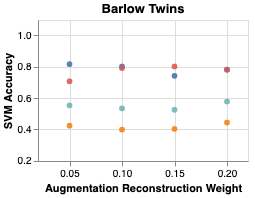
\includegraphics[scale=0.55]{BT_SVM_ReconsWeight.png}
    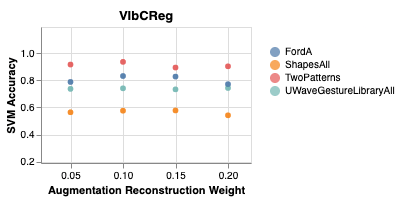
\includegraphics[scale=0.55]{ViB_SVM_ReconsWeight.png}
    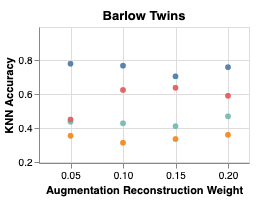
\includegraphics[scale=0.55]{BT_KNN_ReconsWeight.png}
    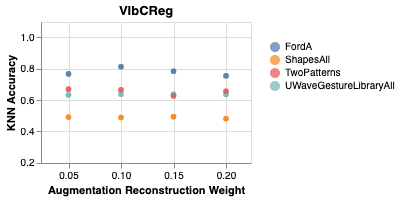
\includegraphics[scale=0.55]{ViB_KNN_ReconsWeight.png}
    \centering  
    \caption{Augmentations: Window Warp and amplitude resize. Averaged across 2 runs. Trained for 250 epochs}  
\end{figure}

\begin{figure}[h]
    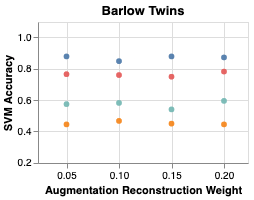
\includegraphics[scale=0.55]{BT_SVM_ReconsWeight_Slice.png}
    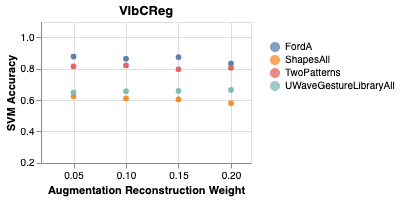
\includegraphics[scale=0.55]{ViB_SVM_ReconsWeight_Slice.png}
    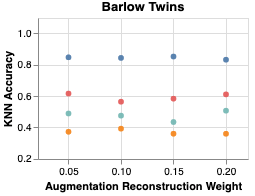
\includegraphics[scale=0.55]{BT_KNN_ReconsWeight_Slice.png}
    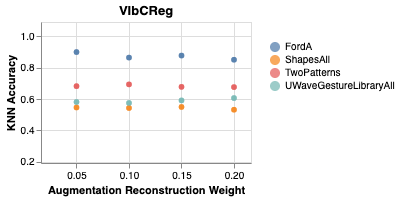
\includegraphics[scale=0.55]{ViB_KNN_ReconsWeight_Slice.png}

    % \centering  
    \caption{Augmentation: Slice and shuffle. Averaged across 2 runs. Trained for 250 epochs}  
\end{figure}

\begin{figure}[h]
    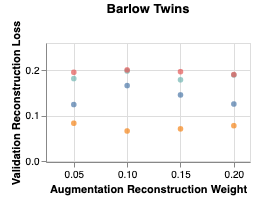
\includegraphics[scale=0.55]{BT_ValRecons_ReconsWeight.png}
    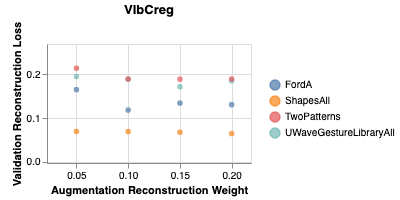
\includegraphics[scale=0.55]{ViB_ValRecons_ReconsWeight.png}
    % \centering  
    \caption{Augmentation: Window Warp and amplitude resize. Averaged across 2 runs. Trained for 250 epochs}  
\end{figure}
\begin{figure}[h]
    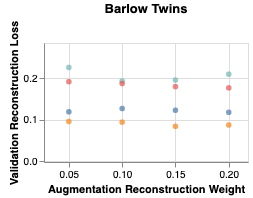
\includegraphics[scale=0.55]{BT_ValRecons_ReconsWeight_Slice.png}
    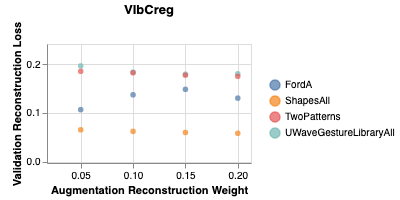
\includegraphics[scale=0.55]{ViB_ValRecons_ReconsWeight_Slice.png}
    % \centering  
    \caption{Augmentation: Slice and shuffle. Averaged across 2 runs. Trained for 250 epochs}  
\end{figure}
\subsection{Augmentation robustness}

S1 - S2 - Augs: Choose datasets such that half were thought to be well fitting for slice and shuffle and half for amplitude resize + window Warp. This was after seeing FordA/B performing well with S&S, and looking at the augmented views.\newline
FordA/B, Electric devices, ShapesALL for S&S\newline
TwoP, UWave, symbols, Mallar for ampRes + winwarp\newline

Visual inspection: Plot training samples + spectrogram, compare to augmented view. Compare these against others from other classes. \newline
Does the resulting improvement in stage 1 transfer to stage 2? 

\TODO{Download the Wandb data.}
Plot for each dataset and each augmentation: 
Color code according to SSL-model.







\end{document}